\documentclass[11pt]{beamer}

\usepackage{hyperref}
\usepackage{graphicx}
\usepackage{longtable}
\usepackage{amsmath}
\usepackage{mdwlist}
\usepackage{listings}
\usepackage{txfonts}
\usepackage{xspace}
\usepackage{amstext}
\usepackage{amssymb}
\usepackage{stmaryrd}
\usepackage{proof}
\usepackage{multicol}
\usepackage[nodayofweek]{datetime}
\usepackage{etex}
\usepackage[all, cmtip]{xy}

%%%%%%%%%%%%%%%%%%%%%%%%%%%%%%%%%%%%%%%%%%%%%%%%%%%%%%%%%%%%%%%%%%%%%%%%%%%%%
%% Macros

\newcommand{\arrow}[1]{{\color{blue}{#1}}}
\newcommand{\red}[1]{{\color{red}{#1}}}
\newcommand{\blue}[1]{{\color{blue}{#1}}}
\newcommand{\timesarr}{\otimes}
\newcommand{\plusarr}{\oplus}
\newcommand{\lcal}{\ensuremath{\lambda}-calculus\xspace}

\def\newblock{}

\newenvironment{floatrule}
    {\hrule width \hsize height .33pt \vspace{.5pc}}
    {\par\addvspace{.5pc}}

%%%%%%%%%%%%%%%%%%%%%%%%%%%%%%%%%%%%%%%%%%%%%%%%%%%%%%%%%%%%%%%%%%%%%%%%%%%%%

%subcode-inline{bnf-inline} name langRev
%! swap+ = \mathit{swap}^+
%! swap* = \mathit{swap}^*
%! dagger =  ^{\dagger}
%! assocl+ = \mathit{assocl}^+
%! assocr+ = \mathit{assocr}^+
%! assocl* = \mathit{assocl}^*
%! assocr* = \mathit{assocr}^*
%! identr* = \mathit{uniti}
%! identl* = \mathit{unite}
%! identr+ = \mathit{zeroi}
%! identl+ = \mathit{zeroe}
%! dist = \mathit{distrib}
%! factor = \mathit{factor}
%! trace+ = \mathit{trace}^+
%! trace* = \mathit{trace}^*
%! :-* = \multimap
%! eta = \eta
%! eps = \epsilon
%! eta+ = \eta^+
%! eps+ = \epsilon^+
%! eta* = \eta
%! eps* = \epsilon
%! (o) = \fatsemi
%! (;) = \fatsemi
%! (*) = \times
%! (+) = +

%subcode-inline{bnf-inline} name langArr
%! arr = \arrow{arr}
%! >>> = ~\arrow{\ggg\xspace}~
%! *** = ~\arrow{\otimes}~
%! +++ = ~\arrow{\oplus}~
%! create = \arrow{create}
%! erase = \arrow{erase}
%! afirst = \arrow{first}
%! asecond = \arrow{second}
%! aleft = \arrow{left}
%! atrace = \arrow{traceA}
%! fstA = \arrow{fstA}
%! sndA = \arrow{sndA}
%! leftA = \arrow{leftA}
%! rightA = \arrow{rightA}
%! |-->>* = \mapsto_{\mathsf{ML}}^{\ast}
%! |-->> = \mapsto_{\mathsf{ML}}

%subcode-inline{bnf-inline} regex \{\{(((\}[^\}])|[^\}])*)\}\} name main include langRev, langArr
%! Gx = \Gamma^{\times}
%! G = \Gamma
%! |-->* = \mapsto^{\ast}
%! |-->> = \mapsto_{\ggg}
%! |-->let = \mapsto_{let}
%! |--> = \mapsto
%! |- = \vdash
%! ==> = \Longrightarrow
%! <=> = \Longleftrightarrow
%! <--> = \rightleftharpoons
%! <-> = \leftrightarrow
%! ~~> = \rightharpoonup
%! ~> = \leadsto
%! ::= = &::=&
%! /= = \neq
%! trans = \mathcal{T}
%! trans1 = \mathcal{T}_1
%! trans2 = \mathcal{T}_2
%! forall = \forall
%! exists = \exists
%! empty = \epsilon
%! least = \phi
%! {[ = \{
%! ]} = \}
%! bottom = \bot
%! alpha = \alpha
%! beta = \beta
%! rho = \rho
%! dagger = ^\dagger
%! @@ = \mu
%! STLC = \lambda^{\rightarrow}
%! STLClet = \textsf{LET}
%! STLCfor = \textsf{LET}^{o}
%! langArr = \textsf{ML}_{\Pi}
%! langArrT = \textsf{ML}_{\Pi^o}
%! langRev = \Pi
%! langRevT = \Pi^{o}
%! langRevEE = \Pi^{\eta\epsilon}
%! if = \mathbf{if}
%! do = \mathbf{do}
%! then = \mathbf{then}
%! else = \mathbf{else}
%! * = \times

\usetheme{Boadilla}

\title{Fractional Types}
\author{Roshan P. James \and Zachary Sparks \\ ~ \\ Jacques Carette (McMaster Univ.) 
\\ ~ \\ Amr Sabry}
\institute{}

\date{February 15, 2013}

\begin{document}

\maketitle

%%%%%%%%%%%%%%%%%%%%%%%%%%%%%%%%%%%%%%%%%%%%%%%%%%%%%%%%%%%%%%%%%%%%%%%%%
\begin{frame}{}

\vfill
{\Large \centerline{The Evil Equal Sign}}

\vfill

\pause

{\Large \centerline{Yes this one \qquad $=$}}
\vfill

\end{frame}

%%%%%%%%%%%%%%%%%%%%%%%%%%%%%%%%%%%%%%%%%%%%%%%%%%%%%%%%%%%%%%%%%%%%%%%%%
\begin{frame}{Equality in Physics}

\begin{itemize}

\vfill\item Take your favorite physical law

\vfill\item $F = m a$

\vfill\item $F$ is the force, obviously. It is one physical \emph{observable}

\vfill\item $m a$ is the rate of change of momentum. It is \red{another}
physical \emph{observable}

\vfill\item Now why and how could two \red{different} physical observables be
\red{equal}

\vfill\item Or, what does it even mean to say that two \red{different} things
are \red{the same}?

\end{itemize}

\vfill

\end{frame}

%%%%%%%%%%%%%%%%%%%%%%%%%%%%%%%%%%%%%%%%%%%%%%%%%%%%%%%%%%%%%%%%%%%%%%%%%
\begin{frame}{Feynman, Landauer, Fredkin, and others}

\begin{itemize}

\vfill\item For centuries, it seemed nobody cared too much

\vfill\item Then computer science came and many people wanted to interpret
the laws of physics computationally, even if only to simulate them.

\vfill\item Argument was made that it is more appropriate to think that
\red{different} observables are related by an \red{isomorphism} and \red{not}
an equality.

\vfill\item We have an isomorphism that \red{witnesses}, \red{explains}, and
\red{models} the \red{process} of transforming one observable to another.

\end{itemize}

\vfill

\end{frame}

%%%%%%%%%%%%%%%%%%%%%%%%%%%%%%%%%%%%%%%%%%%%%%%%%%%%%%%%%%%%%%%%%%%%%%%%%
\begin{frame}{Equality in Mathematics and Logic (\blue{Prehistory})}

\begin{itemize}

\vfill\item Curry-Howard isomorphism: logic, propositions, and
  proofs have computational content.

\vfill\item The statement $e_1 = e_2$ requires proof. 

\vfill\item The statement $e_1 = e_2$ is a computation.

\end{itemize}

\vfill

\end{frame}

%%%%%%%%%%%%%%%%%%%%%%%%%%%%%%%%%%%%%%%%%%%%%%%%%%%%%%%%%%%%%%%%%%%%%%%%%
\begin{frame}{Equality in Mathematics and Logic (\blue{History})}

\begin{itemize}

\vfill\item Martin-L\"of type theory as a foundation for
  constructive mathematics: a \red{computable set theory} if you wish

\vfill\item A crucial component of constructive type theory is \red{equality
  types}: given two terms $e_1, e_2 : A$, we have the \red{type}
$\textit{Id}(e_1,e_2)$ whose canonical inhabitant is $\mathit{refl} :
\textit{Id}(e,e)$.

\vfill\item A term of type $\textit{Id}(e_1,e_2)$ \red{witnesses},
\red{explains}, and \red{models} the process of transforming $e_1$ to $e_2$
and vice-versa.

\vfill\item If you've used Coq or Agda, you know what I am talking about

\end{itemize}

\vfill

\end{frame}

%%%%%%%%%%%%%%%%%%%%%%%%%%%%%%%%%%%%%%%%%%%%%%%%%%%%%%%%%%%%%%%%%%%%%%%%%
\begin{frame}{Equality in Mathematics and Logic (\blue{New Program})}

\begin{itemize}

  \vfill\item \red{Homotopy version of Martin-L\"of Type Theory} or
  \red{Groupoid Interpretation of Martin-L\"of Type Theory}

\vfill\item Classical definition of homotopy: ``two functions are homotopic
if one can be continuously deformed into the other''

\vfill\item Not only do we care about the existence of a proof to show that
two things are equal but we want this proof to be ``smooth'' and
``elementary'' in some sense

\vfill\item Isomorphisms upon isomorphisms upon isomorphisms. Let me explain
using \pause category theory

\end{itemize}

\vfill

\end{frame}

%%%%%%%%%%%%%%%%%%%%%%%%%%%%%%%%%%%%%%%%%%%%%%%%%%%%%%%%%%%%%%%%%%%%%%%%%
\begin{frame}{Category Theory}

A category consists of:

\begin{itemize}

\vfill\item a class of objects;

\vfill\item a class of morphisms; each morphism has a source object and a
target object

\vfill\item a binary operation $\circ$ called composition of morphisms 

\end{itemize}

such that \ldots

\vfill Before we get to the axioms, note that \red{isomorphism} is a central
notion in category theory; most categorical constructions cannot distinguish
between isomorphic objects

\vfill

\end{frame}

%%%%%%%%%%%%%%%%%%%%%%%%%%%%%%%%%%%%%%%%%%%%%%%%%%%%%%%%%%%%%%%%%%%%%%%%%
\begin{frame}{Axioms of a Category}

\begin{itemize}

\vfill\item \red{Associativity}: if $f : A \rightarrow B$, $g : B
  \rightarrow C$, and $h : C \rightarrow D$, then $h \circ (g \circ f) = 
  (h \circ g) \circ f$.

\vfill\item \red{Identity}: for every object $A$, there exists a morphism 
  $\mathit{id}_A : A \rightarrow A$ such that for every morphism 
  $f : A \rightarrow B$, we have 
  $\mathit{id}_B \circ f = f = f \circ \mathit{id}_A$.

\end{itemize}

\vfill

\pause Any questions, comments, or observations?

\vfill

\end{frame}

%%%%%%%%%%%%%%%%%%%%%%%%%%%%%%%%%%%%%%%%%%%%%%%%%%%%%%%%%%%%%%%%%%%%%%%%%
\begin{frame}{$n$-categories}

\begin{itemize}

\vfill\item The equality signs in the axioms should have really really
  really annoyed you. What do they even mean? Equality where and how?

\vfill\item Get rid of these equalities and replace them by isomorphisms.

\vfill\item The morphisms $\mathit{id}_A$, $\mathit{id}_B$, $f$, $g$, $h$
above become \red{objects} in a second-level category and the equality is now
expressed as morphisms between these objects.

\pause 

\vfill\item In English, we now have: $\texttt{Id}_{\texttt{Id}_A(a,b)}(p,q)$

\vfill\item Of course we can iterate this idea

\end{itemize}

\vfill

\end{frame}

%%%%%%%%%%%%%%%%%%%%%%%%%%%%%%%%%%%%%%%%%%%%%%%%%%%%%%%%%%%%%%%%%%%%%%%%%
\begin{frame}{Goal: Develop a Computational Model}

\begin{itemize}

\vfill\item You might ask: why? 

\vfill\item How is this related to anything ``\red{useful}''?

\vfill\item Reason I: most important for me personally: \red{Aesthetics!}
\blue{(Symmetry)}

\vfill\item Meta-reason: ``being in tune with the universe'' is likely to
produce long, lasting, and significant contributions to science

\vfill\item ``Practical'' reasons, coming next

\end{itemize}

\vfill

\end{frame}

%%%%%%%%%%%%%%%%%%%%%%%%%%%%%%%%%%%%%%%%%%%%%%%%%%%%%%%%%%%%%%%%%%%%%%%%%
\begin{frame}{Why Computing with Isomorphisms?}

\begin{itemize}

\vfill\item Programs execution conserves ``resources''; a better linear logic

\vfill\item Programs obey the principle of \red{conservation of information}
(experimental validation of Landauer's principle last year); accidental
information leaks impossible

\vfill\item Program semantics is consistent with the laws of physics:
possible models of quantum, biological, or other emerging ideas

\vfill\item A theory of observation, observational equivalence, that is
itself computational and that does not arbitrarily select a particular set of
equivalences as canonical (e.g., observe assignments to memory but do not
observe memory allocation)

\end{itemize}

\vfill

\end{frame}

%%%%%%%%%%%%%%%%%%%%%%%%%%%%%%%%%%%%%%%%%%%%%%%%%%%%%%%%%%%%%%%%%%%%%%%%%
\begin{frame}{Why Computing with Isomorphisms?}

\begin{itemize}

\vfill\item Type isomorphisms have a long history in PL

\vfill\item First used to \blue{search} libraries: say you are looking for a
function to format a real number to a given number of digits. Does it have type:

{{ Real -> Int -> String}}

{{ Int -> Real -> String}}

{{ Real * Int -> String}}

{{ Int * Real -> String}}

\vfill\item Use equivalence relation on types to query the library with one
of the possible types and get results matching any equivalent type

\vfill\item Related ideas: type isomorphisms allow program reuse, proof
reuse, etc.

\end{itemize}

\vfill

\end{frame}

%%%%%%%%%%%%%%%%%%%%%%%%%%%%%%%%%%%%%%%%%%%%%%%%%%%%%%%%%%%%%%%%%%%%%%%%%
\begin{frame}{}

\vfill
{\Large \centerline{Isomorphisms between Finite Types}}

\vfill

\end{frame}


%%%%%%%%%%%%%%%%%%%%%%%%%%%%%%%%%%%%%%%%%%%%%%%%%%%%%%%%%%%%%%%%%%%%%%%%%
\begin{frame}{Finite Types}

%subcode{bnf} include main
% base types, b ::= 0 | 1 | b+b | b*b 

\begin{itemize}

  \vfill\item 0: no wire

  \vfill\item 1: wire carrying a token {{()}}

  \vfill\item {{b1+b2}}: two wires, one of which carries a value 
  \red{(particle)}

  \vfill\item {{b1*b2}}: two wires, both of which carry a value 
  \red{(wave)}

\end{itemize}

\vfill

\end{frame}

%%%%%%%%%%%%%%%%%%%%%%%%%%%%%%%%%%%%%%%%%%%%%%%%%%%%%%%%%%%%%%%%%%%%%%%%%
\begin{frame}{Graphical notation: Wires} 

\begin{itemize}
\item The simplest sort of diagram is the {{id : b <-> b}} 
\end{itemize}

\begin{multicols}{2}
\begin{center}
\scalebox{0.95}{
\includegraphics{diagrams/thesis/b-wire.pdf}
}
\end{center}
\begin{center}
\scalebox{0.95}{
\includegraphics{diagrams/thesis/b-wire-value.pdf}
}
\end{center}
\end{multicols}

\end{frame}

%%%%%%%%%%%%%%%%%%%%%%%%%%%%%%%%%%%%%%%%%%%%%%%%%%%%%%%%%%%%%%%%%%%%%%%%%
\begin{frame}{Graphical notation: Products} 

\begin{itemize}
\item The product type {{b1*b2}} may be represented using either one wire labeled
{{b1*b2}} or two parallel wires labeled {{b1}} and {{b2}}. 
\end{itemize}

\begin{multicols}{2}
\begin{center}
\scalebox{0.95}{
\includegraphics{diagrams/thesis/product-one-wire.pdf}
}
\end{center}
\begin{center}
\scalebox{0.95}{
\includegraphics{diagrams/thesis/product-one-wire-value.pdf}
}
\end{center}
\end{multicols}
\vfill
\begin{multicols}{2}
\begin{center}
\scalebox{0.95}{
\includegraphics{diagrams/thesis/product-two-wires.pdf}
}
\end{center}
\begin{center}
\scalebox{0.95}{
\includegraphics{diagrams/thesis/product-two-wires-value.pdf}
}
\end{center}
\end{multicols}
\end{frame}

%%%%%%%%%%%%%%%%%%%%%%%%%%%%%%%%%%%%%%%%%%%%%%%%%%%%%%%%%%%%%%%%%%%%%%%%%
\begin{frame}{Graphical notation: Sums} 

\begin{itemize}
\item  Sum types may similarly be represented by one wire or using
  parallel wires with a {{+}} operator between them. 
\end{itemize}

\begin{multicols}{2}
\begin{center}
\scalebox{0.95}{
\includegraphics{diagrams/thesis/sum-one-wire.pdf}
}
\end{center}
\begin{center}
\scalebox{0.95}{
\includegraphics{diagrams/thesis/sum-two-wires-left-value.pdf}
}
\end{center}
\end{multicols}
\vfill
\begin{multicols}{2}
\begin{center}
\scalebox{0.95}{
\includegraphics{diagrams/thesis/sum-two-wires.pdf}
}
\end{center}
\begin{center}
\scalebox{0.95}{
\includegraphics{diagrams/thesis/sum-two-wires-right-value.pdf}
}
\end{center}
\end{multicols}

\end{frame}

%%%%%%%%%%%%%%%%%%%%%%%%%%%%%%%%%%%%%%%%%%%%%%%%%%%%%%%%%%%%%%%%%%%%%%%%%
\begin{frame}{Isomorphisms for Finite Types}

\begin{itemize}

  \vfill\item What are the sound and complete type isomorphisms for
  this system? 

  \vfill\item Folklore that the axioms of a \red{commutative semiring}
  constitute a sound and complete set of type isomorphisms. 

  \vfill\item Proof in LICS 2002 (Balat, Di Cosmo, and Fiore) 

\end{itemize}

\vfill

\end{frame}

%%%%%%%%%%%%%%%%%%%%%%%%%%%%%%%%%%%%%%%%%%%%%%%%%%%%%%%%%%%%%%%%%%%%%%%%%
\begin{frame}{Sound and Complete Isomorphisms}

{\scriptsize
%subcode{bnf} include main
% 0 + b &<->& b // identity for~ +
% b1 + b2 &<->& b2 + b1 // commutativity for~ +
% b1 + (b2 + b3) &<->& (b1 + b2) + b3 // associativity for~ +
}
\pause

{\scriptsize
%subcode{bnf} include main
% 1 * b &<->& b // identity for~ *
% b1 * b2 &<->& b2 * b1 // commutativity for~ *
% b1 * (b2 * b3) &<->& (b1 * b2) * b3 //associativity for~ *
}
\pause

{\scriptsize
%subcode{bnf} include main
% 0 * b &<->& 0 // 0 annihilates
% (b1 + b2) * b3 &<->& (b1 * b3) + (b2 * b3) // distribute over~ +
}

\pause

{\scriptsize
%subcode{proof} include main
%@ ~
%@@ b1 <-> b1
%
%@ b1 <-> b2
%@@ b2 <-> b1
%
%@ b1 <-> b2
%@ b2 <-> b3
%@@ b1 <-> b3
%
%@ equivalence
%
%---
%@ b1 <-> b3
%@ b2 <-> b4
%@@ (b1 + b2) <-> (b3 + b4) 
%
%@ b1 <-> b3
%@ b2 <-> b4
%@@ (b1 * b2) <-> (b3 * b4)
%
%@ congruence
%
}
\end{frame}

%%%%%%%%%%%%%%%%%%%%%%%%%%%%%%%%%%%%%%%%%%%%%%%%%%%%%%%%%%%%%%%%%%%%%%%%%
\begin{frame}{Graphical notation: Associativity} 

\begin{itemize}
\item Associativity is implicit in the graphical language. Three parallel
  wires represent {{b1*(b2*b3)}} or {{(b1*b2)*b3}}, based on the context.
\end{itemize}

\begin{center}
\scalebox{0.95}{
\includegraphics{diagrams/thesis/assoc.pdf}
}
\end{center}

\end{frame}

%%%%%%%%%%%%%%%%%%%%%%%%%%%%%%%%%%%%%%%%%%%%%%%%%%%%%%%%%%%%%%%%%%%%%%%%%
\begin{frame}{Graphical notation: Commutativity} 

\begin{itemize}
\item Commutativity is represented by crisscrossing wires.
\end{itemize}

\begin{multicols}{2}
\begin{center}
\scalebox{0.95}{
\includegraphics{diagrams/thesis/swap_times.pdf}
}
\end{center}
\begin{center}
\scalebox{0.95}{
\includegraphics{diagrams/thesis/swap_plus.pdf}
}
\end{center}
\end{multicols}

\vfill

\begin{multicols}{2}
\begin{center}
\scalebox{0.95}{
\includegraphics{diagrams/thesis/swap_times_value.pdf}
}
\end{center}
\begin{center}
\scalebox{0.95}{
\includegraphics{diagrams/thesis/swap_plus_value.pdf}
}
\end{center}
\end{multicols}

\end{frame}

%%%%%%%%%%%%%%%%%%%%%%%%%%%%%%%%%%%%%%%%%%%%%%%%%%%%%%%%%%%%%%%%%%%%%%%%%
\begin{frame}{Graphical notation: Distributivity and Factoring} 

\begin{itemize}
\item   Distributivity and factoring are represented using the dual boxes shown
  below:
\end{itemize}

\begin{multicols}{2}
\begin{center}
  \includegraphics{diagrams/thesis/dist.pdf}
\end{center}
\begin{center}
  \includegraphics{diagrams/thesis/factor.pdf}
\end{center}
\end{multicols}

\vfill

\begin{multicols}{2}
\begin{center}
  \includegraphics{diagrams/thesis/dist-wire-value1.pdf}
\end{center}
\begin{center}
  \includegraphics{diagrams/thesis/dist-wire-value2.pdf}
\end{center}
\end{multicols}

\end{frame}


%%%%%%%%%%%%%%%%%%%%%%%%%%%%%%%%%%%%%%%%%%%%%%%%%%%%%%%%%%%%%%%%%%%%%%%%%
\begin{frame}{Categorical Interlude}

\begin{itemize}

  \vfill\item A symmetric bimonoidal category

  \vfill\item A symmetric monoidal category $(0,\oplus)$

  \vfill\item A symmetric monoidal category $(1,\otimes)$

  \vfill\item The tensor $\otimes$ distributes over $\oplus$ (\red{but
    not vice-versa}).

  \vfill\item Categorical models of linear logic, quantum computing,
  knot theory, etc. are based on such categories.

\end{itemize} 

\vfill

\end{frame}

%%%%%%%%%%%%%%%%%%%%%%%%%%%%%%%%%%%%%%%%%%%%%%%%%%%%%%%%%%%%%%%%%%%%%%%%%
\begin{frame}{A Reversible Language {{langRev}} }

\begin{itemize}

  \vfill\item A textual notation for the previous diagrams

  \vfill\item Can express all functions on booleans (by embedding them
  in reversible functions)

  \vfill\item With recursion, can express any Turing computable function

\end{itemize} 

\vfill

\end{frame}

%%%%%%%%%%%%%%%%%%%%%%%%%%%%%%%%%%%%%%%%%%%%%%%%%%%%%%%%%%%%%%%%%%%%%%%%%
\begin{frame}
\frametitle{Programming in {{langRev}}: Booleans, Negation}

\vfill

\begin{itemize}
\item We encode booleans by \red{ {{bool = 1 + 1}} } 

{{~~~~~~~~~~~~true = left ()}} 

{{~~~~~~~~~~~~false = right ()}}

\vfill

\item Negation:

\begin{multicols}{2}
\begin{center}
  \includegraphics{diagrams/thesis/swap_plus.pdf}
\end{center}

\begin{center}
  \includegraphics{diagrams/thesis/swap_plus_value.pdf}
\end{center}
  
\end{multicols}

\vfill 

    {{~~~~~~ not : bool <-> bool }}

    {{~~~~~~ not = swap+}} 
\end{itemize}

\vfill

\end{frame}

%%%%%%%%%%%%%%%%%%%%%%%%%%%%%%%%%%%%%%%%%%%%%%%%%%%%%%%%%%%%%%%%%%%%%%%%%%
\begin{frame}{Programming in {{langRev}}: Conditionals}
  
\begin{itemize}

\item Reversible conditional:
{{ if_c (flag, b) = if flag then (flag, c(b)) else (flag, b) }}

\vfill

\item Given {{c : b <-> b}}, then:

{{if_c : bool * b <-> bool * b }}

{{ if_c = dist (;) ((id (*) c) (+) id) (;) factor}}

\vfill

\begin{center}
  \includegraphics{diagrams/thesis/cnot.pdf}
\end{center}

\vfill
\end{itemize}

\end{frame}

%%%%%%%%%%%%%%%%%%%%%%%%%%%%%%%%%%%%%%%%%%%%%%%%%%%%%%%%%%%%%%%%%%%%%%%%%
\begin{frame}{Recursion}

\begin{itemize}

\vfill\item Add \red{recursive types} (so that we can now define
natural numbers, lists, trees, etc.)

\vfill\item Add categorical \red{trace} (the categorical abstraction
of \red{feedback}, \red{looping}, and \red{recursion})

\vfill

\begin{center}
  \includegraphics{diagrams/trace_plus.pdf}
\end{center}

\vfill

\end{itemize}

\end{frame}


%%%%%%%%%%%%%%%%%%%%%%%%%%%%%%%%%%%%%%%%%%%%%%%%%%%%%%%%%%%%%%%%%%%%%%%%%
\begin{frame}{}

\vfill
{\Large \centerline{Higher-Order Extension}}

\vfill

\end{frame}

%%%%%%%%%%%%%%%%%%%%%%%%%%%%%%%%%%%%%%%%%%%%%%%%%%%%%%%%%%%%%%%%%%%%%%%%%
\begin{frame}{Extending the language {{langRevEE}} } 

\begin{itemize}
\vfill\item Processes can observe other processes

\vfill\item Proofs of equalities can themselves be compared for equality

\vfill\item Generally useful to have functions as values; code-as-data;
data-as-code

\end{itemize}

\vfill

\end{frame}

%%%%%%%%%%%%%%%%%%%%%%%%%%%%%%%%%%%%%%%%%%%%%%%%%%%%%%%%%%%%%%%%%%%%%%%%%
\begin{frame}{Negative Information}

\begin{itemize}
  \vfill\item Introduce the idea of \red{negative information} or
  \red{request} for information; 

  \vfill\item Information is logarithmic: entropy of a random variable of
  drawn from a set of size {{N}} is {{ {@1@ log N @} }}. 

  \vfill\item To get {{ {@1@ -log N @} }} information, we need to set of
  ``size'' {{1/N}}.

  \vfill\item Assume these sets exist for now \ldots and let's add
  \red{fractional} types and values.

\end{itemize}

\vfill

\end{frame}

%%%%%%%%%%%%%%%%%%%%%%%%%%%%%%%%%%%%%%%%%%%%%%%%%%%%%%%%%%%%%%%%%%%%%%%%%
\begin{frame}{Extending the language {{langRevEE}} } 

\begin{itemize}
\vfill\item Types
%subcode{bnf} include main
% base types, b ::= 0 | 1 | b+b | b*b | {@1@ 1/b @}
\vfill\item Isomorphisms
%subcode{opsem} include main
% eta* &: 1 <-> (1/b) * b :& eps*
\end{itemize}

\vfill

Let's remove the {{0}} to avoid some potential subtle problems with division
by {{0}} (whatever that means at the level of types)

\end{frame}

%%%%%%%%%%%%%%%%%%%%%%%%%%%%%%%%%%%%%%%%%%%%%%%%%%%%%%%%%%%%%%%%%%%%%%%%%
\begin{frame}
\frametitle{Multiplicative Duality}

\begin{multicols}{2}
\begin{center}
\scalebox{1.5}{
  \includegraphics{diagrams/eta_times1.pdf}
}
\end{center}

\begin{center}
\scalebox{1.5}{
  \includegraphics{diagrams/eps_times1.pdf}
}
\end{center}  
\end{multicols}

\end{frame}

%%%%%%%%%%%%%%%%%%%%%%%%%%%%%%%%%%%%%%%%%%%%%%%%%%%%%%%%%%%%%%%%%%%%%%%%%
\begin{frame}{Sanity Checks}

\begin{itemize}
  \vfill\item Idea of negative information makes sense in a world in which
  information is conserved;

\vfill\item Can ``borrow'' because the infrastructure guarantees that all
debts must be accounted for;

\vfill\item Sets with fractional size do exist! \red{Intuition:} Consider an
object with a symmetry group of size {{N}}. If you are counting naively you
will count this object {{N}} times but all these counts are ``the
same''. Divide by {{N}} to get the ``real count''.

\end{itemize}

\end{frame}

%%%%%%%%%%%%%%%%%%%%%%%%%%%%%%%%%%%%%%%%%%%%%%%%%%%%%%%%%%%%%%%%%%%%%%%%%
\begin{frame}{Homotopy Cardinality or Groupoid Cardinality}

\begin{itemize}
\vfill\item Formally this idea is known as \red{homotopy cardinality} or
  \red{groupoid} cardinality

\vfill\item That exactly what the ``new program'' in type theory is all
  about

\vfill\item In type theory, the intuition is that a statement may have
  several proofs but we don't want to count all the proofs as different, so 
  we divide by the size of the equivalence class of all proofs

  \vfill\item Anyway, it seems that we are on a sound footing. Lots of
  details to work out tough! For now, let's have fun and program with these
  fractional types. What can we do with them?

\end{itemize}

\end{frame}

%%%%%%%%%%%%%%%%%%%%%%%%%%%%%%%%%%%%%%%%%%%%%%%%%%%%%%%%%%%%%%%%%%%%%%%%%
\begin{frame}{Programming with Fractional Types and Values}

\begin{itemize}
\vfill\item Introduce the abbreviation: {{ b1 :-* b2 = 1/b1 * b2}}

\vfill\item We can turn an isomorphism {{b1 <-> b2}} into a value:

%subcode{opsem} include main
%! columnStyle = rcl
% name &:& (b1 <-> b2) -> (1 <-> (b1 :-* b2))
% name c &=& eta*_{b1} (;) (id (*) c)

\vfill\item We can express recursion:

%subcode{opsem} include main
%! columnStyle = rcl
% trace*_b &:& ((b * b1) <-> (b * b2)) -> (b1 <-> b2)
% trace*_b c &=& uniti (;) (eta*_b (*) id) (;) assocr* (;) 
%            && (id (*) c) (;) assocl* (;) (eps*_b (*) id) (;) unite

\end{itemize}

\vfill

\end{frame}

%%%%%%%%%%%%%%%%%%%%%%%%%%%%%%%%%%%%%%%%%%%%%%%%%%%%%%%%%%%%%%%%%%%%%%%%%
\begin{frame}{Programming with Fractional Types and Values}

\begin{itemize}

\vfill\item We can apply and compose these higher-order relations:

%subcode{opsem} include main
%! columnStyle = rcl
% apply &:& (b1 :-* b2) * b1 <-> b2
% apply &=& swap* (;) assocl* (;) (swap* (*) id) (;) (eps*_{b1} (*) id) (;) unite
% 
% compose &:& (b1 :-* b2) * (b2 :-* b3) -> (b1 :-* b3)
% compose &=& assocr* (;) 
%   && (id (*) (assocl* (;) (swap* (*) id) (;) (eps*_{b2} (*) id) (;) unite))

\end{itemize}

\vfill

\end{frame}

%%%%%%%%%%%%%%%%%%%%%%%%%%%%%%%%%%%%%%%%%%%%%%%%%%%%%%%%%%%%%%%%%%%%%%%%%
\begin{frame}{More Intuitively: Duality}

\begin{center}
\scalebox{1.0}{
  \includegraphics{diagrams/coherence.pdf} 
}
\end{center}

\end{frame}

%%%%%%%%%%%%%%%%%%%%%%%%%%%%%%%%%%%%%%%%%%%%%%%%%%%%%%%%%%%%%%%%%%%%%%%%%
\begin{frame}{More Intuitively: Functions}

\begin{center}
\scalebox{1.5}{
  \includegraphics{diagrams/function.pdf}
}
\end{center}

\end{frame}

%%%%%%%%%%%%%%%%%%%%%%%%%%%%%%%%%%%%%%%%%%%%%%%%%%%%%%%%%%%%%%%%%%%%%%%%%
\begin{frame}{More Intuitively}

\begin{center}
\scalebox{1.5}{
  \includegraphics{diagrams/compose1.pdf}
}
\end{center}

\end{frame}

%%%%%%%%%%%%%%%%%%%%%%%%%%%%%%%%%%%%%%%%%%%%%%%%%%%%%%%%%%%%%%%%%%%%%%%%%
\begin{frame}{More Intuitively}

\begin{center}
\scalebox{1.5}{
  \includegraphics{diagrams/compose.pdf}
}
\pause
\scalebox{1.5}{
  \includegraphics{diagrams/compose2.pdf}
}
\end{center}

\end{frame}

%%%%%%%%%%%%%%%%%%%%%%%%%%%%%%%%%%%%%%%%%%%%%%%%%%%%%%%%%%%%%%%%%%%%%%%%%
\begin{frame}{More Intuitively}

\begin{center}
\scalebox{1.5}{
  \includegraphics{diagrams/apply1.pdf}
}
\end{center}

\end{frame}

%%%%%%%%%%%%%%%%%%%%%%%%%%%%%%%%%%%%%%%%%%%%%%%%%%%%%%%%%%%%%%%%%%%%%%%%%
\begin{frame}{More Intuitively}

\begin{center}
\scalebox{1.5}{
  \includegraphics{diagrams/apply2.pdf}
}
\end{center}

\end{frame}

%%%%%%%%%%%%%%%%%%%%%%%%%%%%%%%%%%%%%%%%%%%%%%%%%%%%%%%%%%%%%%%%%%%%%%%%%
\begin{frame}{SAT Solver}

\begin{center}
\scalebox{1.2}{
  \includegraphics{diagrams/sat2.pdf}
}
\end{center}  

\begin{center}
\scalebox{1.5}{
  \includegraphics{diagrams/sat3.pdf}
}
\end{center}  

\end{frame}

%%%%%%%%%%%%%%%%%%%%%%%%%%%%%%%%%%%%%%%%%%%%%%%%%%%%%%%%%%%%%%%%%%%%%%%%%
\begin{frame}{}

{\Large \centerline{Conclusions --- The Bigger Picture}}

\end{frame}

%%%%%%%%%%%%%%%%%%%%%%%%%%%%%%%%%%%%%%%%%%%%%%%%%%%%%%%%%%%%%%%%%%%%%%%%%
\begin{frame}{Physical Perspective on Computation}

\begin{itemize}

  \vfill\item Computer science abstractions are based on \blue{old}
  physics

  \vfill\item Computer applications are more and more ``physical''

  \vfill\item Physical principles such as \red{conservation of
    information} should be part of our foundational abstractions

  \vfill\item Other principles?

\end{itemize} 

\vfill

\end{frame}

%%%%%%%%%%%%%%%%%%%%%%%%%%%%%%%%%%%%%%%%%%%%%%%%%%%%%%%%%%%%%%%%%%%%%%%%%
\begin{frame}{Computational Perspective on Physics}

\begin{itemize}

  \vfill\item Towards a computational understanding of quantum mechanics

  \vfill\item Creation and annihilation of ``entangled'' particles
  appears fundamental; modeled by computational symmetries and
  dualities

  \vfill\item Negative information flow and negative entropy are
  existing concepts in quantum information

  \vfill\item Discrete Quantum Computing: Take the Hilbert space
  formalism and replace the underlying field of \red{uncomputable}
  complex numbers with a finite field! In the simplest case, we get
  {{langRev}} with one addition: a \red{disjoint union} operation.

\end{itemize} 

\vfill

\end{frame}

%%%%%%%%%%%%%%%%%%%%%%%%%%%%%%%%%%%%%%%%%%%%%%%%%%%%%%%%%%%%%%%%%%%%%%%%%
%%%%%%%%%%%%%%%%%%%%%%%%%%%%%%%%%%%%%%%%%%%%%%%%%%%%%%%%%%%%%%%%%%%%%%%%%

\end{document}


